% oocriterion.tex
\documentclass[main.tex]{subfiles}
\begin{document}
\chapter{Failure Criteria in AM} \label{ch:oocrit}

As described during Section \ref{sec:FC} of Chapter \ref{ch:bg}, currently available failure criteria fail to completely integrate interaction effects into the modeled failure behavior of anisotropic materials. In 2017, Paul and Tim Osswald proposed a model that attempts to overcome these limitiations \cite{Osswald2017a}. This recent failure criterion has the following characteristics:
\begin{itemize}
	\item \textbf{Tensor based and purely mathematical}: as opposed to phenomenological or mechanistic models such as the Puck or Cuntze failure criteria.
	\item \textbf{Based on the Gol'denblat-Kopnov model}.
	\item \textbf{Includes stress interactions that other models neglect}.
\end{itemize}

Originally titled \textquotedblleft A Strength Tensor Based Failure Criterion with Stress Interactions\textquotedblright, it will be referred in this work as the Stress-Stress Interaction Criterion (SSIC). This chapter will briefly describe the Gol'denblat-Kopnov model upon which the SSIC is based, followed by a proper description of how it implements stress interactions. Finally, it will go detail how it was used to develop a failure envelopes for parts produced through AM techniques, focusing on a recent example deployed for FFF parts produced with ABS.

\section{The Gol'denblat-Kopnov Model}\label{sec:GKC}
The Gol'denblat-Kopnov Criterion (GKC) describes a mathematical function that depends on the stress state of an anisotropic material. Should the computation of this expression exceed a threshold, part failure is to be expected. To that end, a scalar function that depends on stress tensors that completely characterize the state of the material was developed \cite{Goldenblat1965}. This function is shown in Equation \ref{eq:GKCgen}, where stresses are denoted $\sigma$, and the subindices \emph{i,j,k,l} denote a particular load direction.

\begin{equation} \label{eq:GKCgen}
f=(F_{ij}\sigma_{ij})^\alpha + (F_{ijkl}\sigma_{ij}\sigma_{kl})^\beta + (F_{ijklmn}\sigma_{ij}\sigma_{kl}\sigma_{mn})^\gamma + ...
\end{equation}

The terms $F_{ij}$, $F_{ijkl}$ and $F_{ijklmn}$ represent second, fourth and sixth order tensors respectively. These terms of the equation depend on engineering strength parameters, such as the ultimate tensile and compressive strengths of the material in a particular load direction \cite{Osswald2017a}. Due to the complexity associated with using higher order tensors, Gol'denblat and Kopnov limited their approach to using only the second and fourth order terms. Thus Equation \ref{eq:GKCgen} is reduced to:

\begin{equation} \label{eq:GKCgenTrunc}
f=(F_{ij}\sigma_{ij})^\alpha + (F_{ijkl}\sigma_{ij}\sigma_{kl})^\beta
\end{equation}

In order to attain a linear criterion scalar function, the exponents $\alpha$ and $\beta$ were assigned values of 1 and 1/2 respectively. Finally, in plane stress scenarios, the GKC becomes:

\begin{equation} \label{eq:GKCfinal}
\begin{split}
f=F_{11}\sigma_{11} + F_{22}\sigma_{22} + F_{12}\tau_{12} + (F_{1111}\sigma_{11}^{2} + F_{2222}\sigma_{22}^{2} + F_{1212}\tau_{12}^{2} \\ + 2F_{1122}\sigma_{11}\sigma_{22} + 2F_{1112}\sigma_{11}\tau_{12} + 2F_{2212}\sigma_{22}\tau_{12})^{1/2}
\end{split}
\end{equation}

Note that in Equation \ref{eq:GKCfinal} $\sigma$ and $\tau$ denote normal and shear stresses respectively. Figure \ref{fig:loaddir} depicts an anisotropic material and all the possible loading directions for reference.

\begin{figure}[h]
	\center
	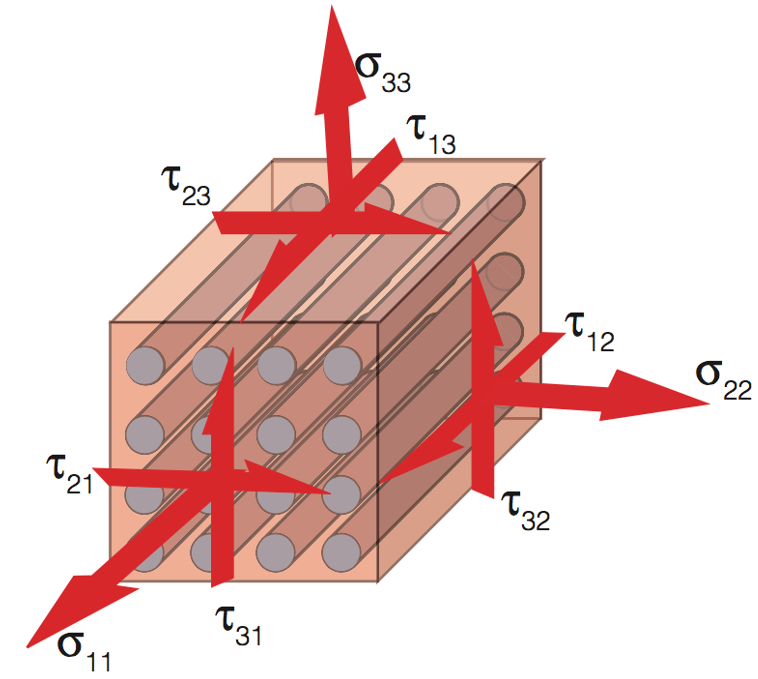
\includegraphics[height=5cm]{reference_cube}
	\caption{Different load directions in an anisotropic material} \label{fig:loaddir}
\end{figure}

Per Gol'denblat and Kopnov's design, should the computation of $f$ in Equation \ref{eq:GKCfinal} be greater or equal to 1, part failure is to be expected. However, to simplify calculations, they deliberately assumed the interaction terms $F_{1112}$ and $F_{2212}$ to be zero. This is an important consideration that will come into play when describing the SSIC.

Most of the terms in the GKC are obtained through mechanical testing of coupons under pure uniaxial loads in the 1 or 2 direction, or pure shear in the 1-2 plane \cite{Osswald2017a}. In these scenarios, $f$ will be equal to 1 at failure, and the stress state will be known to the user, allowing some of the unknown tensorial parameters to be easily calculated. Using $F_{11}$ and $F_{1111}$ as examples, the process would be as follows:
\pagebreak
\begin{enumerate}
	\item The tensile and compressive strength in the 1-1 direction would be obtained through mechanical testing. These values are named $X_t$ and $X_c$ respectively.
	\item Under these failure conditions, Equation \ref{eq:GKCfinal} is reduced to the following system of equations:
	\[
	\systeme*{1=F_{11}X_t + (F_{1111}X_t^{2})^{1/2}, 1= -F_{11}X_c + (F_{1111}X_c^{2})^{1/2}}
	\]

	\item $F_{11}$ and $F_{1111}$ can be obtained, yielding $F_{11}=\frac{1}{2}(\frac{1}{X_t}-\frac{1}{X_c})$ and $F_{1111}=\frac{1}{4}(\frac{1}{X_t}+\frac{1}{X_c})^2$.
\end{enumerate}

The only exception to this procedure would be the $F_{1122}$ component, which requires measuring the positive and negative shear strengths of a coupon with reinforcement oriented in 45$^\circ$. These parameters are named $S_{45p}$ and $S_{45n}$ respectively. Table \ref{tab:GKparam} summarizes the nomenclature used for the strength parameters required to completely populate the failure function of the GKC. Table \ref{tab:GKtens} summarizes all the tensorial component calculations.

\begin{table} [h]
	\centering
	\caption{Nomenclature of the GKC parameters}
	\begin{tabular}{ c c }
	\toprule
		\textbf{Parameter} & \textbf{Description} \\ 
		\midrule
		$X_t$ & Tensile strength in the 1-1 direction\\
		$X_c$ & Compressive strength in the 1-1 direction\\
		$Y_t$ & Tensile strength in the 2-2 direction\\
		$Y_c$ & Compressive strength in the 2-2 direction\\
		$S_{45p}$ & Positive shear strength for 45$^\circ$ specimen\\
		$S_{45n}$ & Negative shear strength for 45$^\circ$ specimen\\
		$S$ & Shear strength in the 1-2 plane\\
	\bottomrule
	\end{tabular}
	\label{tab:GKparam}
\end{table}

\begin{table} [h]
	\centering
	\caption{Tensorial components of the GKC}
	\begin{tabular}{ c c } 
	\toprule
		\textbf{Component} & \textbf{Formula} \\
		\midrule
		$F_{11}$ & $\frac{1}{2}(\frac{1}{X_t}-\frac{1}{X_c})$\\ [1ex]
		$F_{1111}$ & $\frac{1}{4}(\frac{1}{X_t}+\frac{1}{X_c})^2$\\ [1ex]
		$F_{22}$ & $\frac{1}{2}(\frac{1}{Y_t}-\frac{1}{Y_c})$\\ [1ex]
		$F_{2222}$ & $\frac{1}{4}(\frac{1}{Y_t}+\frac{1}{Y_c})^2$\\ [1ex]
		$F_{12}$ & 0\\ [1ex]
		$F_{1212}$ & $\frac{1}{S^2}$\\ [1ex]
		$F_{1122}$ & $\frac{1}{8}[(\frac{1}{X_t}+\frac{1}{X_c})^2+(\frac{1}{Y_t}+\frac{1}{Y_c})^2-(\frac{1}{S_{45p}}+\frac{1}{S_{45n}})^2]$\\ [1ex]
		\bottomrule
	\end{tabular}
	\label{tab:GKtens}
\end{table}
\pagebreak

\section{The Stress-Stress Interaction Criterion}\label{sec:OOC}
One of the assumptions made in the GKC is that the components $F_{1112}$ and $F_{2212}$ in Equation \ref{eq:GKCfinal} are null. While this simplifies the model, it essentially neglects any interactions between axial loads and shear stresses, namely, the $\sigma_{11}$~-~$\tau_{12}$ and $\sigma_{22}$~-~$\tau_{12}$ interactions. Practically, this causes the failure surface developed through the GKC to under-predict shear strengthening effects exhibited by anisotropic materials loaded in combined axial and shear conditions. The Stress-Stress Interaction Criterion (SSIC) attempts to overcome these limitations by building upon the GKC. For the SSIC, the interaction effects are captured through the use of the slopes of the failure surface at any of the points where the engineering strength is known within a particular stress plane \cite{Osswald2017a}. In this failure scenario, the stress state of the coupon is known and easy to implement into Equation \ref{eq:GKCfinal}, where $f=1$. The resulting expression can then be derived with respect to one of the stresses, allowing for the interaction components to be calculated. This is better illustrated through an example. Assuming the component of interest is $F_{2212}$, the procedure to calculate it through the SSIC would be as follows:

\begin{enumerate}
	\item Obtain all the tensorial components possible through the GKC.
	\item Using the $\sigma_{22}$\textendash$\tau_{12}$ stress plane, take the derivative of Equation \ref{eq:GKCfinal} as a function of $\sigma_{22}$ in the scenario of failure under pure shear ($f=1$). This yields the expression:
	\begin{equation} \label{eq:OOCex1}
	 0= F_{22}+[F_{1212}S(\frac{d\tau_{12}}{d\sigma_{22}})+F_{2212}S]
	\end{equation}
	 where $\frac{d\tau_{12}}{d\sigma_{22}}$  is the slope of the graph at failure under shear. This term is named $\mu^{2212}$ in the SSIC and can be obtained by performing combined loading tests. 
	 
	\item Rearranging Equation \ref{eq:OOCex1} to solve for the unknown $F_{2212}$ gives the following expression:
	\begin{equation} \label{eq:OOCex2}
	F_{2212}=-\frac{F_{22}}{S}-F_{1212}\mu^{2212}
	\end{equation}
\end{enumerate}


A similar procedure can be followed for any $\sigma_{ii}$-$\tau_{ij}$ interaction, or even any $\sigma_{ii}$-$\sigma_{jj}$ components. For this last scenario, the user has four potential choices of slopes to determine the tensorial component of interest. In the SSIC, any slope obtained from a $\sigma_{ii}$-$\sigma_{jj}$ stress plane is named $\lambda^{iijj}$, as opposed to $\mu^{iiij}$ for slopes in a $\sigma_{ii}$-$\tau_{ij}$ reference. A schematic of all possible interaction slopes is shown in Figure \ref{fig:SSICdemo}, while Table \ref{tab:OOCcomp} summarizes all the possible interaction factors available through the SSIC, where $\tau_{ij}^u$ denotes ultimate shear strength in a particular shear plane. 

\pagebreak
\begin{figure}[h]
	\center
	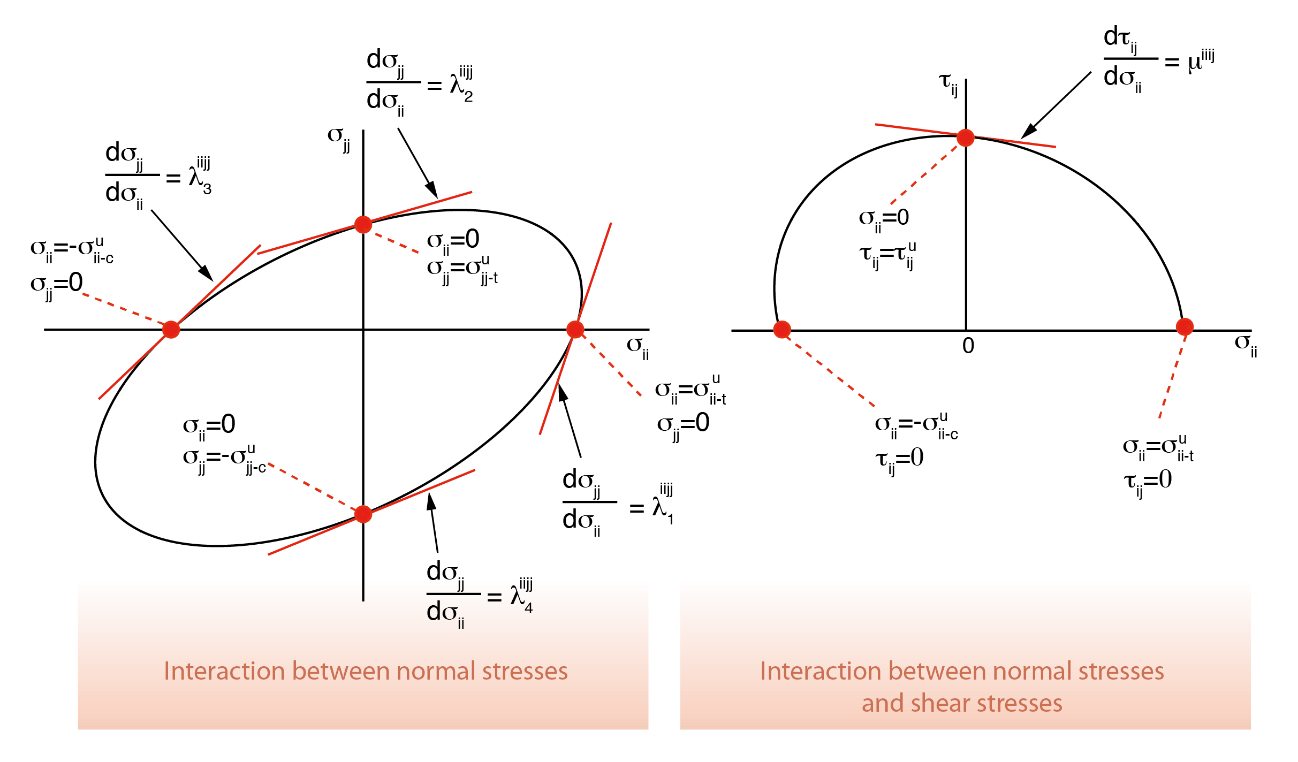
\includegraphics[height=9cm]{ssic_slopes}
	\caption{Interaction slopes available through the SSIC} \label{fig:SSICdemo}
\end{figure}
\begin{table}[!htbp] %Fixates table so that it doesn't randomly jump around between pages
	\renewcommand{\arraystretch}{1.5}
	\centering
	\caption{Interaction components attainable through the SSIC~\cite{Osswald2017a}}
	\begin{tabular}{ c c } 
		\toprule
		\textbf{Component} & \textbf{Formula} \\
		\midrule
		$F_{iiij}$ & $-\frac{F_{ii}}{\tau_{ij}^u}-F_{ijij}\mu^{iiij}$\\
		$F_{iijj}$ through $\lambda^{iijj}_1$ & $-\frac{(F_{ii}+F_{jj}\lambda^{iijj}_1)F_{iiii}^{1/2}+F_{iiii}}{\lambda^{iijj}_1}$\\
		$F_{iijj}$ through $\lambda^{iijj}_2$ & $-(F_{ii}+F_{jj}\lambda^{iijj}_2)F_{jjjj}^{1/2}-F_{jjjj}\lambda^{iijj}_2$\\
		$F_{iijj}$ through $\lambda^{iijj}_3$ & $\frac{(F_{ii}+F_{jj}\lambda^{iijj}_3)F_{iiii}^{1/2}-F_{iiii}}{\lambda^{iijj}_3}$\\
		$F_{iijj}$ through $\lambda^{iijj}_4$ & $(F_{ii}+F_{jj}\lambda^{iijj}_4)F_{jjjj}^{1/2}-F_{jjjj}\lambda^{iijj}_4$\\
		\bottomrule
	\end{tabular}
	\label{tab:OOCcomp}
\end{table}

\subsection{Applications of the SSIC in AM}\label{sec:SSICAM}

The SSIC offers a way of capturing in a more accurate manner the different failure modes of parts produced through AM technologies. As an example, the model has been successfully implemented by Obst \emph{et al.} in 2018 for SLS manufactured parts produced with PA12 \cite{Obst2018, Obst2017}. Their results show how the model was able to capture the $\tau_{12}$-$\sigma_{22}$ and $\sigma_{11}$-$\sigma_{22}$ interactions. The failure surface obtained, shown in Figure \ref{fig:OOCSLS}, was able to capture the interactions between certain axial and transverse stresses. However, due to the limitations of the SLS process, it was not possible to measure the interaction slope between the $\tau_{12}$ and $\sigma_{11}$ directions.

\begin{figure}[h]
	\center
	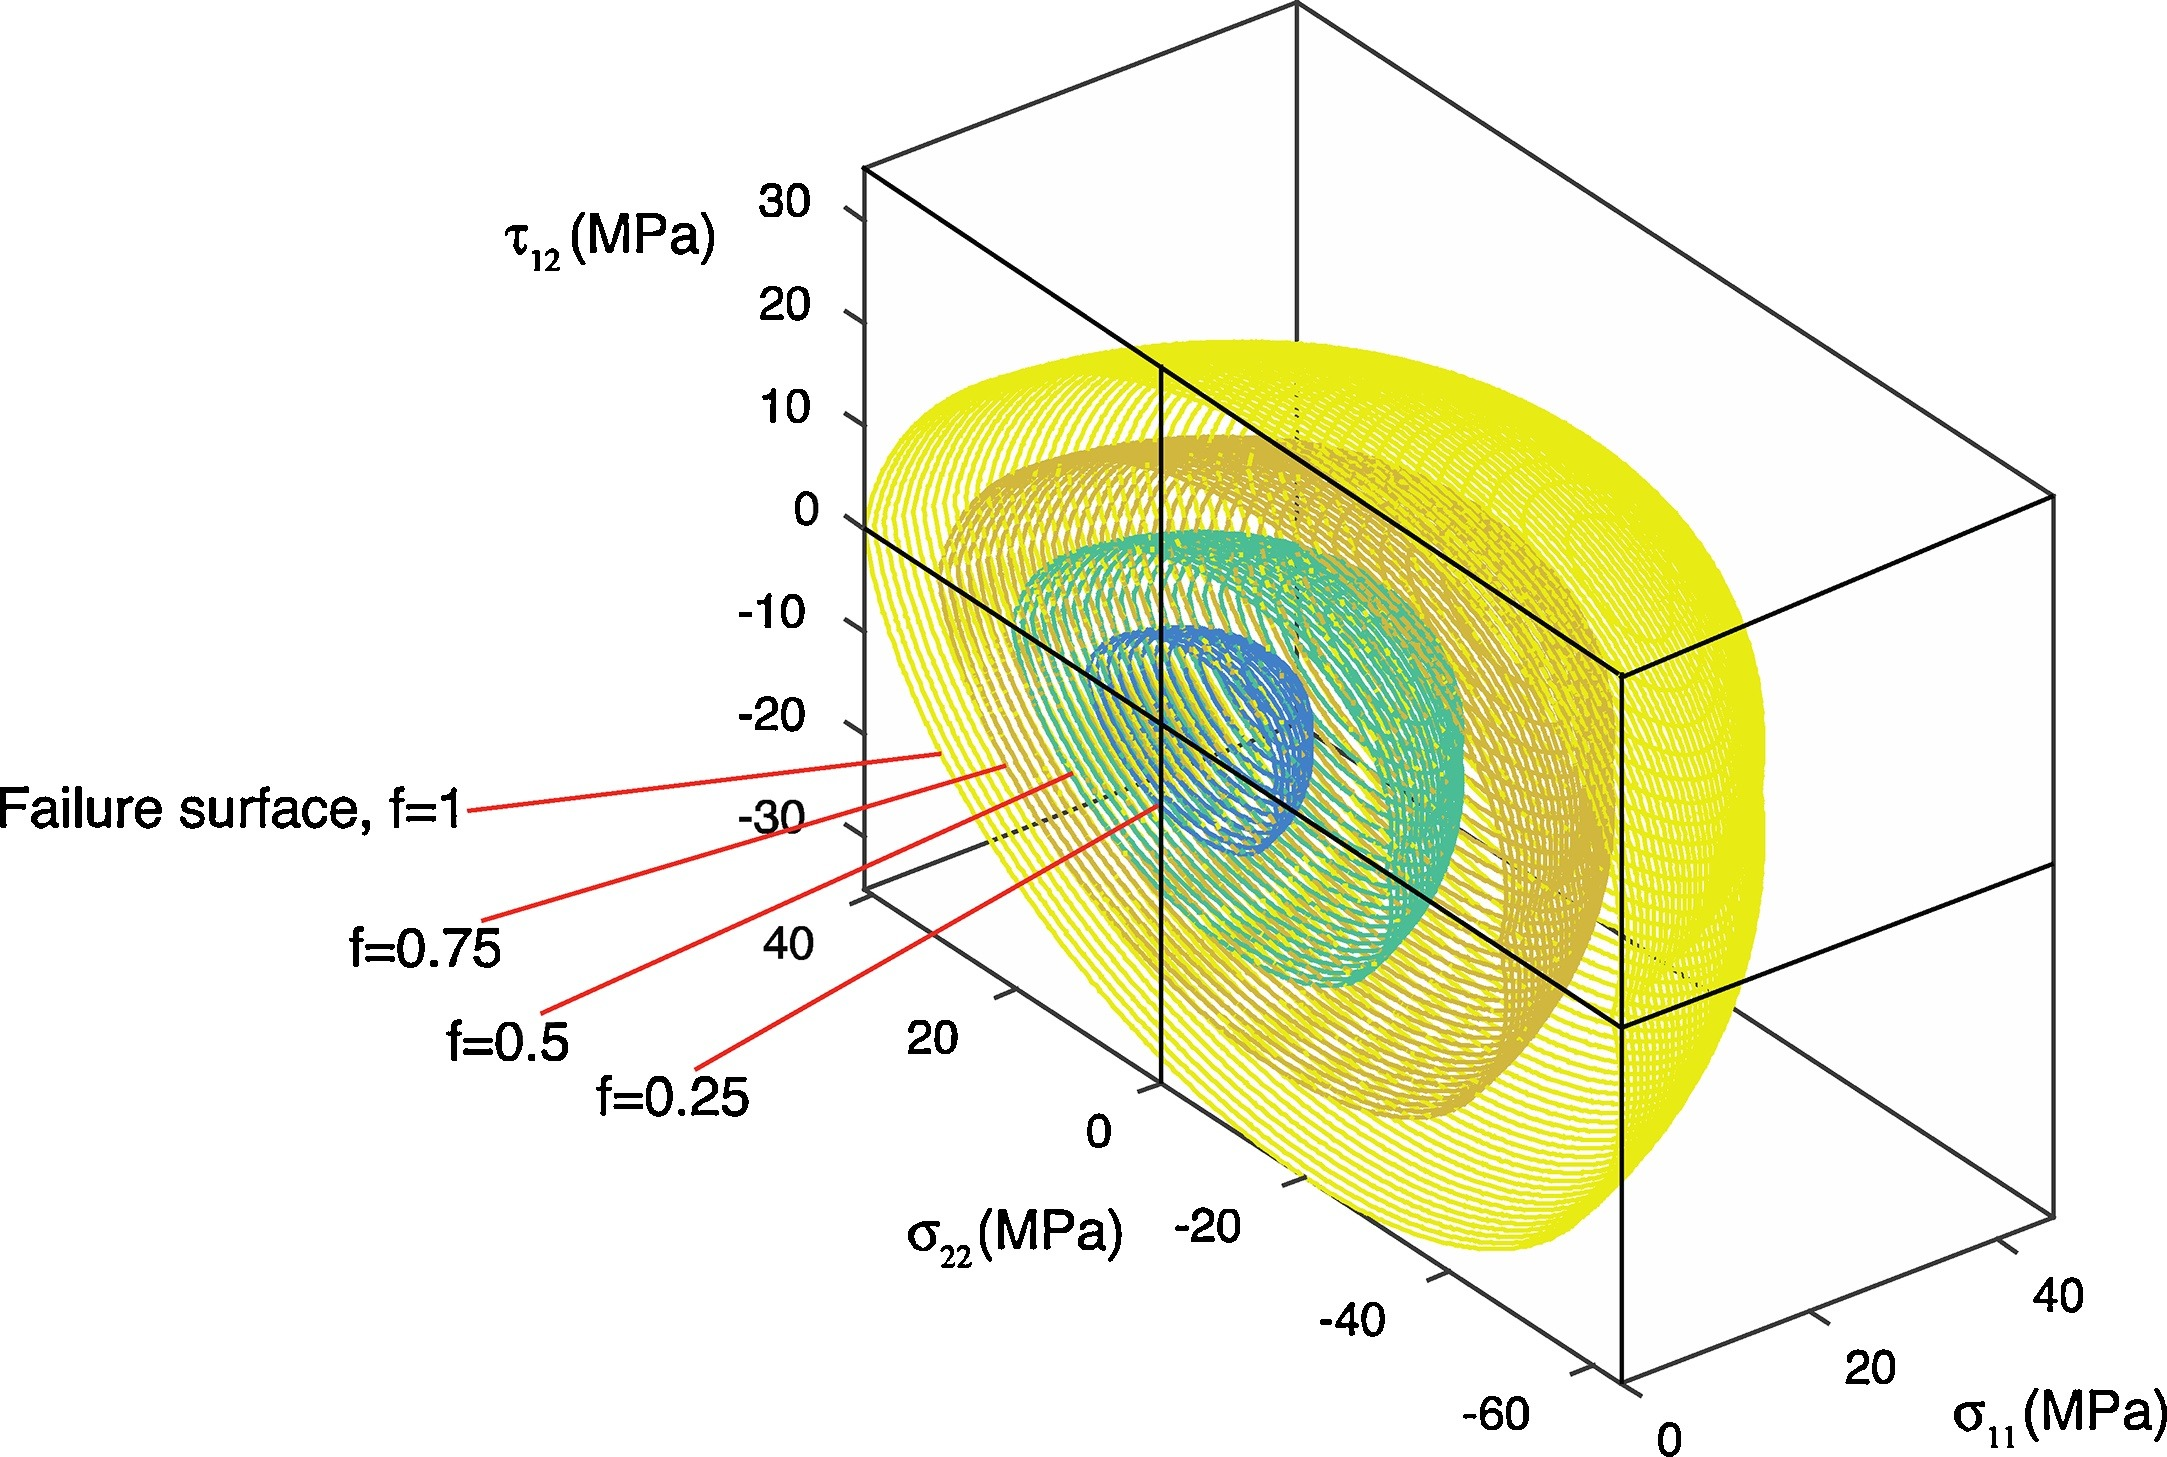
\includegraphics[height=6cm]{Obst_SLS}
	\caption{Failure surface for SLS developed through the SSIC \cite{Obst2018}} \label{fig:OOCSLS}
\end{figure}

Recent unpublished work by Osswald \emph{et al.} \cite{Osswald2020} generated a failure envelope for Multi-Jet Fusion (MJF) parts produced using PA12, and compared it to the surface obtained by Obst \emph{et al.} \cite{Obst2018}. Results indicate that, while both techniques are based on Powder Based Fusion (PBF) and use the same material, the envelopes for each AM technology were distinct, serving as proof that these technologies are not as comparable under complex loading conditions as previously assumed. The transverse-axial interaction for the MJF case was significantly less pronounced than for SLS, further reinforcing that each AM technique needs to be studied in a case-by-case basis in terms of mechanical failure characterization. 

\begin{figure}[!htbp]
	\center
	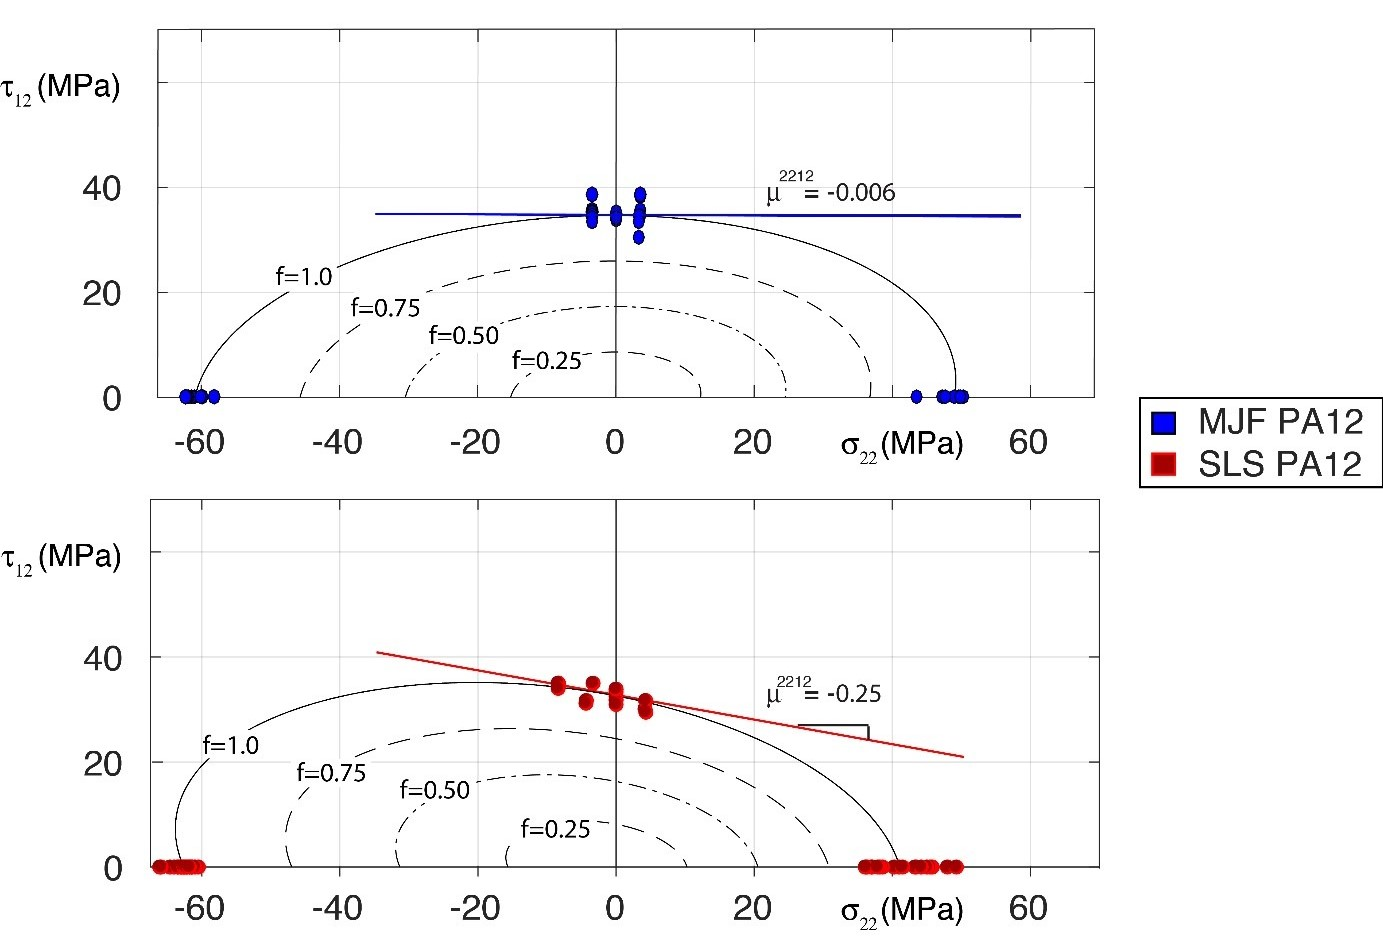
\includegraphics[height=10cm]{pbfcomp}
	\caption{Comparison of the $\sigma_{22} - \tau_{12}$ interaction for SLS and MJF PA12 parts \cite{Osswald2020}} \label{fig:pbfcomp}
\end{figure}

In 2019, Mazzei Capote \emph{et al.} \cite{MazzeiCapote2019} developed a failure envelope for FFF parts produced using a customized ABS filament produced in-house. Specimens were produced using either a commercially available desktop FFF printer (Lulzbot TAZ5, USA), or a customized 6-axis robotic printing solution whenever the bead orientation was hard to achieve using a \emph{2.5-D} machine. The robotic printer was based on a 6-axis robot (ABB IRB-120, Switzerland) and fitted with a stationary printhead mounted on an aluminum frame, chosen to be the same extruder from the traditional printer (LulzBot TAZ Single Extruder Tool Head v2, 0.5 mm nozzle, USA) to minimize machine influence on the results \cite{VanHulle2017}. The final surface obtained showed significant stress interactions in certain directions. Starting with the $\sigma_{11}$-$\sigma_{22}$ plane, it can be seen that the failure envelope has a slight tilt. Refer to Figure~\ref{fig:1122plane} for a graph showing the calculated failure envelope, including the experimental data for reference. This tilt is evidence of an interaction between the transverse and longitudinal stresses. The conclusion is that FFF parts produced with the print parameters used in the study should show strengthening when loaded bi-axially in compression.

\begin{figure}[h]
	\center
	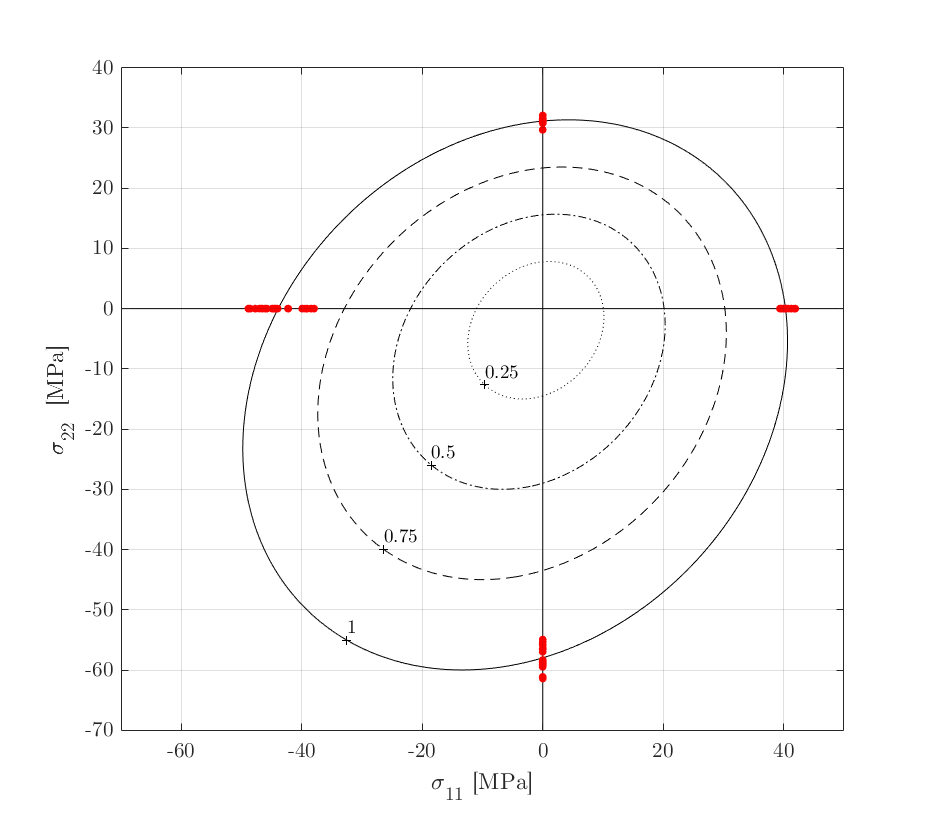
\includegraphics[width=0.9\linewidth, keepaspectratio]{11_22plane}
	\captionsetup{justification=centering} %long caption
	\caption[failure envelope in the $\sigma_{11}$-$\sigma_{22}$ plane]{$\sigma_{11}$-$\sigma_{22}$ plane including data for reference.} \label{fig:1122plane}
\end{figure}

Using the results from combined loading tests plotted in the $11-12$ and $22-12$ planes allows visualization of the transverse-axial stress interactions. Beginning with the $11-12$ plane, it can be seen that the calculated interaction slope $\mu^{1112}$ equals $5.2\times 10^{-3}$, a value that's practically zero. Using this parameter, the failure surface shown in Figure \ref{fig:1112plane} can be obtained. A dashed line representing $\mu^{1112}$ is added for reference. The $22-12$ plane by comparison reveals a considerable slope. It can be seen through the use of combined loads that there is a slight decrease in the shear strength of the specimens when a tensile load is applied in the $2-2$ direction. A slope of -0.2 was obtained for $\mu^{2212}$. Figure \ref{fig:2212plane} shows the resulting surface with the data and a line with a slope of -0.2 overlaid for reference.

\begin{figure}[!htbp]
	\center
	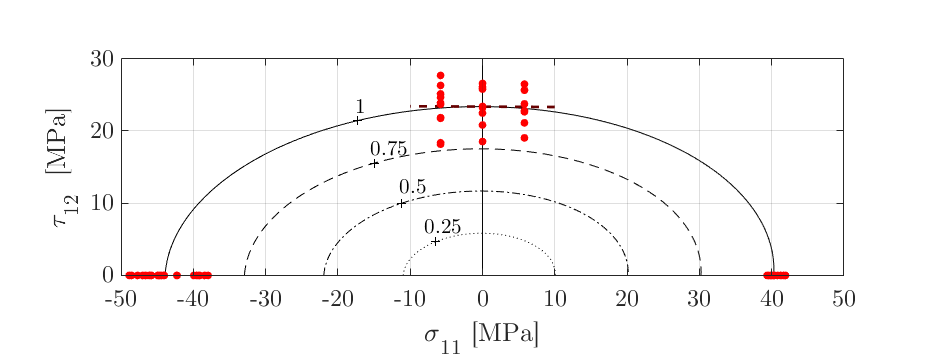
\includegraphics[width=\linewidth, keepaspectratio]{11_12plane}
	\captionsetup{justification=centering} %long caption
	\caption[failure envelope in the $\sigma_{11}$-$\tau_{12}$ plane]{$\sigma_{11}$-$\tau_{12}$ plane including data for reference.} \label{fig:1112plane}
\end{figure}

\begin{figure}[!htbp]
	\center
	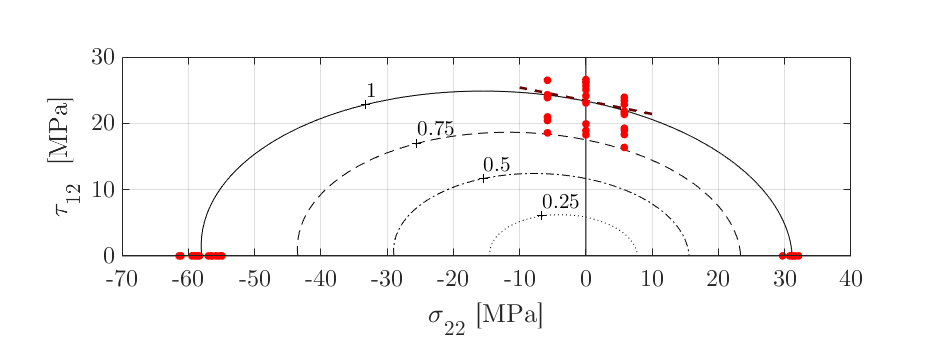
\includegraphics[width=\linewidth, keepaspectratio]{22_12plane}
	\captionsetup{justification=centering} %long caption
	\caption[failure envelope in the $\sigma_{22}$-$\tau_{12}$ plane]{$\sigma_{22}$-$\tau_{12}$ plane including data for reference.} \label{fig:2212plane}
\end{figure}
  


% Nomenclature introduced in this chapter:
\nomenclature[A]{SSIC}{Stress-Stress Interaction Criterion}% 
\nomenclature[A]{GKC}{Gol'denblat-Kopnov Criterion}% 
\nomenclature[A]{MJF}{Multi-Jet Fusion}% 
\nomenclature[A]{PBF}{Powder Bed Fusion}% 

% Symbols introduced in this chapter:
\nomenclature[S]{$X_t$}{Tensile strength in the 1-1 direction \nomunit{$MPa$}}
\nomenclature[S]{$X_c$}{Compressive strength in the 1-1 direction \nomunit{$MPa$}}
\nomenclature[S]{$Y_t$}{Tensile strength in the 2-2 direction \nomunit{$MPa$}}
\nomenclature[S]{$Y_c$}{Compressive strength in the 2-2 direction \nomunit{$MPa$}}
\nomenclature[S]{$S$}{Shear strength in the 1-2 plane \nomunit{$MPa$}}
\nomenclature[S]{$S_{45p}$}{Positive shear strength for 45$^\circ$ specimen \nomunit{$MPa$}}
\nomenclature[S]{$S_{45n}$}{Negative shear strength for 45$^\circ$ specimen \nomunit{$MPa$}}
\nomenclature[S]{$\mu^{1112}$}{SSIC parameter- slope at pure shear failure in the $\sigma_{11}$ - $\tau_{12}$ plane \nomunit{$-$}}
\nomenclature[S]{$\mu^{2212}$}{SSIC parameter- slope at pure shear failure in the $\sigma_{22}$ - $\tau_{12}$ plane \nomunit{$-$}}
\end{document}